\section{\label{sec:total_corr_func} Total correlation functions}
\subsection{Definitions}
The definition of the n-particle distribution function is taken from \cite{HANSEN2013ch2} (see Eq.~(2.6.7) therein)
\begin{equation}
\label{def:g_n}
g^{(n)}(\vb{r}^n)=\frac{\rho^{(n)}(\vb{r}_1,\dotsc,\vb{r}_n)}{\prod_{i=1}^{n}\rho^{(1)}(\vb{r}_i)}
\end{equation}
where $\rho^{(n)}$ is the n-particle density (see Eq.~(2.6.1) in \cite{HANSEN2013ch2}), which is defined as:
\begin{eqnarray}
	\label{def:rho_n}
	\rho^{(n)}(\vb r^n) = \frac{1}{\Xi}\sum_{N=n}^{\infty} \frac{z^N}{(N-n)!} \int\exp(-\beta U_N) d\vb r^{(N-n)}
\end{eqnarray}
Here $\vb r^n \equiv \vb r_1, \dotsc, \vb r_n$, and $d\vb r^{(N-n)} = d\vb r_{n+1} \dotsc d\vb r_N$.

Let's introduce an hierarchy of total correlation functions. The most widely known element of this hierarchy is the pair correlation function
\begin{equation}
\label{def:pair_corr_func}
h^{(2)}(\vb{r}_1,\vb{r}_2) = g^{(2)}(\vb{r}_1,\vb{r}_2) - 1
\end{equation}
(e.g., see Eq.~(2.6.8) in~\cite{HANSEN2013ch2}).

Let's express the total correlation functions in terms of the n-particle distribution functions.
Formally, one can introduce the hierarchy of total correlation functions starting from $n=1$ and on.
By definition
\begin{equation}
g^{(1)}(\vb{r})\equiv 1.
\end{equation}
Thus, for $n=1$ one has: 
\begin{equation}
h^{(1)}(\vb{r}) = g^{(1)}(\vb{r}) = 1.
\end{equation}

For $n=2$:
\begin{equation}
h^{(2)}(\vb{r}_1,\vb{r}_2) = g^{(2)}(\vb{r}_1,\vb{r}_2) - 1
\end{equation}

For $n=3$:
\begin{eqnarray}
h^{(3)}(\vb{r}_1 ,\vb{r}_2, \vb{r}_3) &=& g^{(3)}(\vb{r}_1, \vb{r}_2, \vb{r}_3) - g^{(2)}(\vb{r}_1, \vb{r}_2) 
\nonumber\\
&&-g^{(2)}(\vb{r}_1,\vb{r}_3) -  g^{(2)}(\vb{r}_2,\vb{r}_3) +2.
\end{eqnarray}

For $n=4$ :
\begin{eqnarray}
h^{(4)}(\vb{r}_1, \vb{r}_2, \vb{r}_3, \vb{r}_4) &=& g^{(4)}(\vb{r}_1, \vb{r}_2, \vb{r}_3, \vb{r}_4) - g^{(3)}(\vb{r}_1, \vb{r}_2, \vb{r}_3) 
\nonumber\\
&&-g^{(3)}(\vb{r}_1, \vb{r}_2, \vb{r}_4) -  g^{(3)}(\vb{r}_1, \vb{r}_3, \vb{r}_4) - g^{(3)}(\vb{r}_2, \vb{r}_3, \vb{r}_4) 
\nonumber\\
&&-g^{(2)}(\vb{r}_1,\vb{r}_2) g^{(2)}(\vb{r}_3,\vb{r}_4) - g^{(2)}(\vb{r}_1,\vb{r}_3) g^{(2)}(\vb{r}_2,\vb{r}_4) - g^{(2)}(\vb{r}_1,\vb{r}_4)g^{(2)}(\vb{r}_2,\vb{r}_3)
\nonumber\\
&&+2(g^{(2)}(\vb{r}_1,\vb{r}_2) + g^{(2)}(\vb{r}_1,\vb{r}_3) + g^{(2)}(\vb{r}_1,\vb{r}_4)
\nonumber\\
&&+g^{(2)}(\vb{r}_2,\vb{r}_3) + g^{(2)}(\vb{r}_2,\vb{r}_4) + g^{(2)}(\vb{r}_3,\vb{r}_4)) 
\nonumber\\
&&-6.
\end{eqnarray}

\subsection{Expressed via $g^{(n)}$ and $h^{(m<n)}$}
The total correlation functions $h^{(n)}$ can be expressed via $g^{(n)}$ and $h^{(m<n)}$.
Such representation for total correlation functions $h^{(3)}$ and $h^{(4)}$ was used in \cite{attardJCP1990}.

For $n=3$:
\begin{eqnarray}
h^{(3)}(\vb{r}_1 ,\vb{r}_2, \vb{r}_3) &=& g^{(3)}(\vb{r}_1, \vb{r}_2, \vb{r}_3) - h^{(2)}(\vb{r}_1, \vb{r}_2) 
\nonumber\\
&&-h^{(2)}(\vb{r}_1,\vb{r}_3) -  h^{(2)}(\vb{r}_2,\vb{r}_3) -1.
\end{eqnarray}

For $n=4$:
\begin{eqnarray}
h^{(4)}(\vb{r}_1, \vb{r}_2, \vb{r}_3, \vb{r}_4) &=& g^{(4)}(\vb{r}_1, \vb{r}_2, \vb{r}_3, \vb{r}_4) - h^{(3)}(\vb{r}_1, \vb{r}_2, \vb{r}_3) 
\nonumber\\
&&-h^{(3)}(\vb{r}_1, \vb{r}_2, \vb{r}_4) -  h^{(3)}(\vb{r}_1, \vb{r}_3, \vb{r}_4) - h^{(3)}(\vb{r}_2, \vb{r}_3, \vb{r}_4) 
\nonumber\\
&&-h^{(2)}(\vb{r}_1,\vb{r}_2) h^{(2)}(\vb{r}_3,\vb{r}_4) - h^{(2)}(\vb{r}_1,\vb{r}_3) h^{(2)}(\vb{r}_2,\vb{r}_4) - h^{(2)}(\vb{r}_1,\vb{r}_4)h^{(2)}(\vb{r}_2,\vb{r}_3)
\nonumber\\
&&-h^{(2)}(\vb{r}_1,\vb{r}_2) - h^{(2)}(\vb{r}_1,\vb{r}_3) - h^{(2)}(\vb{r}_1,\vb{r}_4)
\nonumber\\
&&-h^{(2)}(\vb{r}_2,\vb{r}_3) - h^{(2)}(\vb{r}_2,\vb{r}_4) - h^{(2)}(\vb{r}_3,\vb{r}_4) 
\nonumber\\
&&-1.
\end{eqnarray}

From here it's straightforward to express $g^{(n)}$ via $h^{(m)}$, where $m \leq n$ (in \cite{hernandoPRA1986} such expressions were presented for $n\leq3$).

\subsection{Expressed via $g^{(n)}$ through $g^{(1)}$}
For $n=2$:
\begin{eqnarray}
h^{(2)}(\vb{r}_1,\vb{r}_2) = g^{(2)}(\vb{r}_1,\vb{r}_2) - g^{(1)}(\vb{r}_1) g^{(1)}(\vb{r}_2)
\end{eqnarray}

For $n=3$:
\begin{eqnarray}
h^{(3)}(\vb{r}_1 ,\vb{r}_2, \vb{r}_3) &=& g^{(3)}(\vb{r}_1, \vb{r}_2, \vb{r}_3) - g^{(2)}(\vb{r}_1, \vb{r}_2) g^{(1)}(\vb{r}_3)
\nonumber\\
&&-g^{(2)}(\vb{r}_1,\vb{r}_3) g^{(1)}(\vb{r}_2) -  g^{(2)}(\vb{r}_2,\vb{r}_3) g^{(1)}(\vb{r}_1)
\nonumber\\
&& +2g^{(1)}(\vb{r}_1)g^{(1)}(\vb{r}_2)g^{(1)}(\vb{r}_3).
\end{eqnarray}

For $n=4$ :
\begin{eqnarray}
h^{(4)}(\vb{r}_1, \vb{r}_2, \vb{r}_3, \vb{r}_4) &=& g^{(4)}(\vb{r}_1, \vb{r}_2, \vb{r}_3, \vb{r}_4) - g^{(3)}(\vb{r}_1, \vb{r}_2, \vb{r}_3) g^{(1)}(\vb{r}_4)
\nonumber\\
&&-g^{(3)}(\vb{r}_1, \vb{r}_2, \vb{r}_4) g^{(1)}(\vb{r}_3) -  g^{(3)}(\vb{r}_1, \vb{r}_3, \vb{r}_4) g^{(1)}(\vb{r}_2) - g^{(3)}(\vb{r}_2, \vb{r}_3, \vb{r}_4)g^{(1)}(\vb{r}_1) 
\nonumber\\
&&-g^{(2)}(\vb{r}_1,\vb{r}_2) g^{(2)}(\vb{r}_3,\vb{r}_4) - g^{(2)}(\vb{r}_1,\vb{r}_3) g^{(2)}(\vb{r}_2,\vb{r}_4) - g^{(2)}(\vb{r}_1,\vb{r}_4)g^{(2)}(\vb{r}_2,\vb{r}_3)
\nonumber\\
&& + 2[g^{(2)}(\vb{r}_1,\vb{r}_2)g^{(1)}(\vb{r}_3) g^{(1)}(\vb{r}_4) + g^{(2)}(\vb{r}_1,\vb{r}_3) g^{(1)}(\vb{r}_2) g^{(1)}(\vb{r}_4) 
\nonumber\\
&& + g^{(2)}(\vb{r}_1,\vb{r}_4)g^{(1)}(\vb{r}_2)g^{(1)}(\vb{r}_3) + g^{(2)}(\vb{r}_2,\vb{r}_3)g^{(1)}(\vb{r}_2) g^{(1)}(\vb{r}_4)
\nonumber\\
&& + g^{(2)}(\vb{r}_2,\vb{r}_4)g^{(1)}(\vb{r}_1) g^{(1)}(\vb{r}_3) + g^{(2)}(\vb{r}_3,\vb{r}_4)g^{(1)}(\vb{r}_1) g^{(1)}(\vb{r}_2) ]
\nonumber\\
&&-6g^{(1)}(\vb{r}_1) g^{(1)}(\vb{r}_2)g^{(1)}(\vb{r}_3) g^{(1)}(\vb{r}_4).
\end{eqnarray}

Equivalent representations for n-point correlation functions were used in \cite{white1979} in research on galaxy clustering.

To simplify notation, let's denote $(\vb{r}_1, \dotsc, \vb{r}_n) = (1, \dotsc, n)$. And let's group similar terms under summation sings.
Then $h^{(3)}$ and $h^{(4)}$ can be rewritten as
\begin{eqnarray}
h^{(3)}(1,2,3) &=& g^{(3)}(1, 2, 3) 
- \sum_{\vb l = \left\{\substack{1,2,3 \\ 1,3,2 \\ 2,3,1} \right\} } g^{(2)}(l_1,l_2) g^{(1)}(l_3)
\nonumber\\
&& +2g^{(1)}(1)g^{(1)}(2)g^{(1)}(3).
\end{eqnarray}
\begin{eqnarray}
h^{(4)}(1,2,3,4) &=& g^{(4)}(1,2,3,4) 
- \sum_{\vb l = \left\{\substack{1,2,3,4 \\ 1,2,4,3 \\ 1,3,4,2 \\ 2,3,4,1}\right\} }g^{(3)}(l_1,l_2,l_3) g^{(1)}(l_4) 
\nonumber\\
&&-\sum_{\vb l = \left\{ \substack{1,2,3,4 \\ 1,3,2,4 \\ 1,4,2,3} \right\}}g^{(2)}(l_1,l_2) g^{(2)}(l_3,l_4)
\nonumber\\
&& + 2\sum_{\vb l = \left\{\substack{1,2,3,4 \\ 1,3,2,4 \\ 1,4,2,3 \\ 2,3,1,4 \\ 2,4,1,3 \\ 3,4,1,2} \right\}} g^{(2)}(l_1,l_2)g^{(1)}(l_3) g^{(1)}(l_4) 
\nonumber\\
&&-6g^{(1)}(1) g^{(1)}(2)g^{(1)}(3) g^{(1)}(4).
\end{eqnarray}

The sums extend over all distinct argument lists in which each point appears exactly once. E.g. $g^{(3)}(1,2,3)$ and $g^{(3)}(3,2,1)$ are not considered distinct, and terms such as $g^{(2)}(1,2)g^{(2)}(2,3)$ do not appear \cite{white1979}.

\subsection{Fourier components of total correlation functions}
The following generic notation is used for the Fourier components of the total correlation function:
\begin{equation}
\hat{h}^{(n)}(\vb{k}_1,\dotsc, \vb{k}_n) = \int \exp(-i\vb{k}_1\vb{r}_1 - \dotsc - i\vb{k}_n\vb{r}_n) h^{(n)}(\vb{r}_1, \dotsc, \vb{r}_n) d\vb{r}_1\dotsc d\vb{r}_n
\end{equation}
By properly selecting the origin, it can be shown that for a homogeneous isotropic system:
\begin{equation}
g^{(n)}(\vb{r}_1, \dotsc, \vb{r}_n) = g^{(n)}(\vb{r}_1 - \vb{r}_n, \dotsc, \vb{r}_{n-1} - \vb{r}_{n})
\end{equation}
and applying a proper change of variables it can be written as:
\begin{equation}
g^{(n)} = g^{(n)}(\vb{r}_1, \dotsc, \vb{r}_{n-1})
\end{equation}
Thus,
\begin{equation}
h^{(n)}(\vb{r}_1, \dotsc, \vb{r}_n) \Rightarrow h^{(n)}(\vb{r}_1, \dotsc, \vb{r}_{n-1})
\end{equation}

It enables us to write the following expressions for the Fourier components $\hat{h}^{(n)} (\vb{k}^n)$:
\begin{equation}
\frac{1}{V}\hat{h}^{(n)} (\vb{k}^n) = \hat{h}^{(n)} (\vb{k}_1, \dotsc, \vb{k}_{n-1}) 
\delta_{\vb{k}_1+\dotsc + \vb{k}_n}
\end{equation}
where
\begin{equation}
\hat{h}^{(n)}(\vb{k}_1, \dotsc, \vb{k}_{n-1}) = \int \exp(-i\vb{k}_1\vb{r}_1 - \dotsc - i\vb{k}_{n-1}\vb{r}_{n-1}) h^{(n)}(\vb{r}_1, \dotsc, \vb{r}_{n-1})d\vb{r}_1\dotsc d\vb{r}_{n-1}
\end{equation}

In particular, for $n=1$:
\begin{equation}
\hat{h}^{(1)}(\vb{k}) = \int \exp(-i\vb{k}\vb{r})h^{(1)}(\vb{r})d\vb{r} = \int \exp(-i\vb{k}\vb{r})d\vb{r}
\end{equation}
\begin{equation}
\frac{1}{V}\hat{h}^{(1)}(\vb{k}) = \delta_{\vb{k}}
\end{equation}

For $n=2$:
\begin{equation}
\frac{1}{V}\hat{h}^{(2)}(\vb{k}_1, \vb{k}_2) = \hat{h}^{(2)}(\vb{k}_1)\delta_{\vb{k}_1 + \vb{k}_2}
\end{equation}

\subsection{Fourier transform of the radial correlation function for the hard-spheres system}
From~\cite{Ashcroft1966} (see Eqs.~(3)-(5) therein) an explicit expression for $\hat{h}^{(2)}(k)$ can be calculated in the Percus-Yevick approximation.
Figure~\ref{h2_vs_k} shows the dependency of $\hat{h}^{(2)}(k)/\sigma^3$ on $k \sigma$. Figure~\ref{h2_vs_eta} shows the dependency of $\hat{h}^{(2)}(0)/\sigma^3$ on packing fraction $\eta.$
\begin{figure}[htbp]
	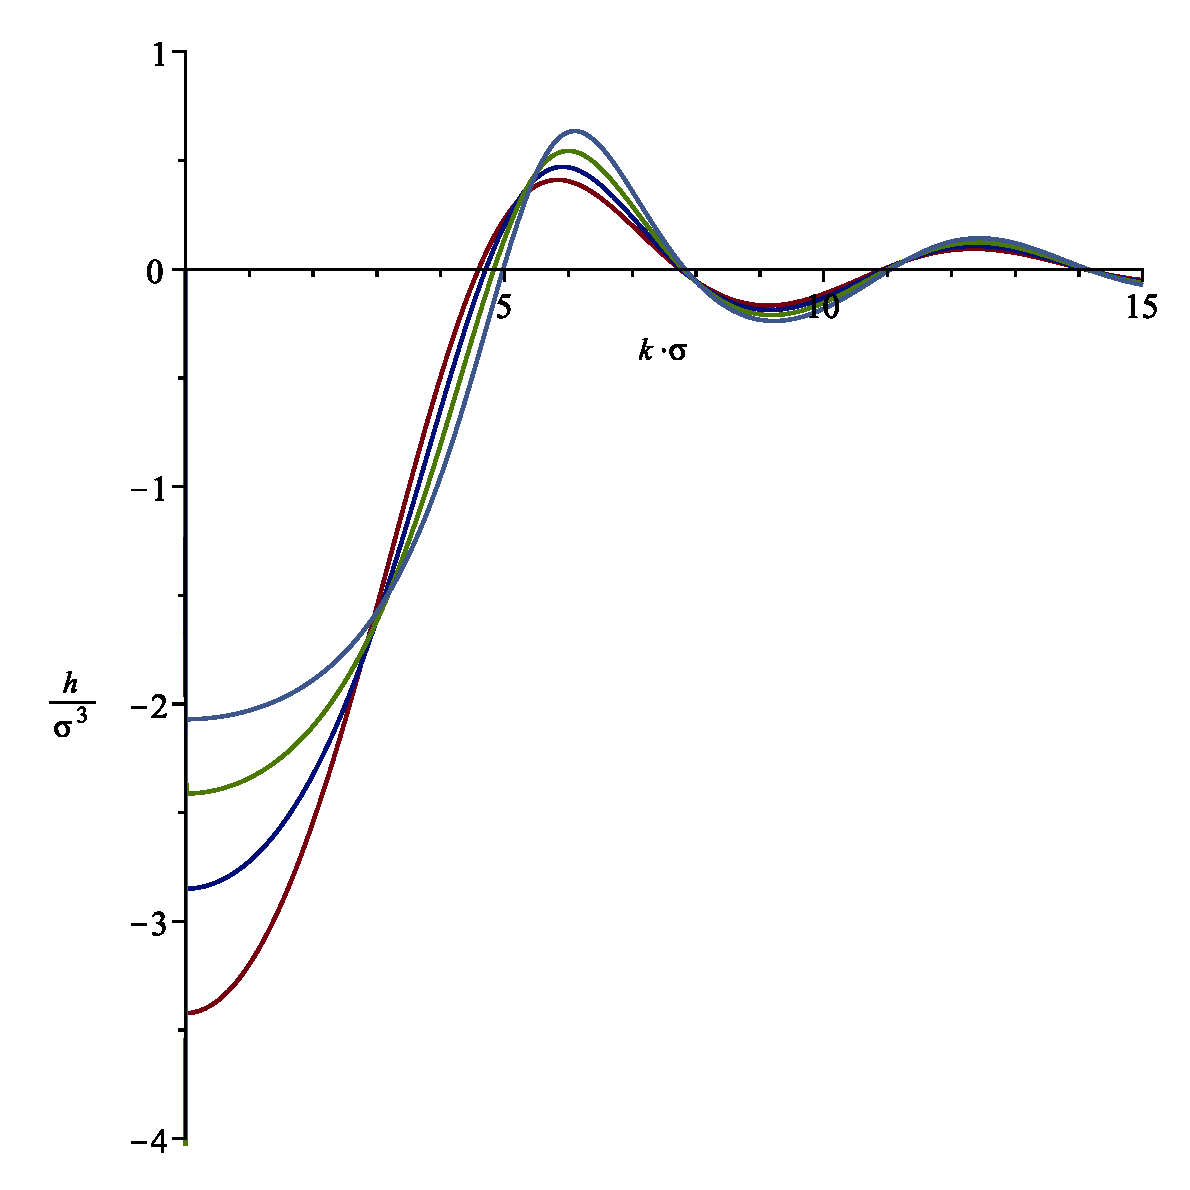
\includegraphics[width=0.45\textwidth,angle=0]{h2_as_function_of_k_at_different_eta} \hfill
	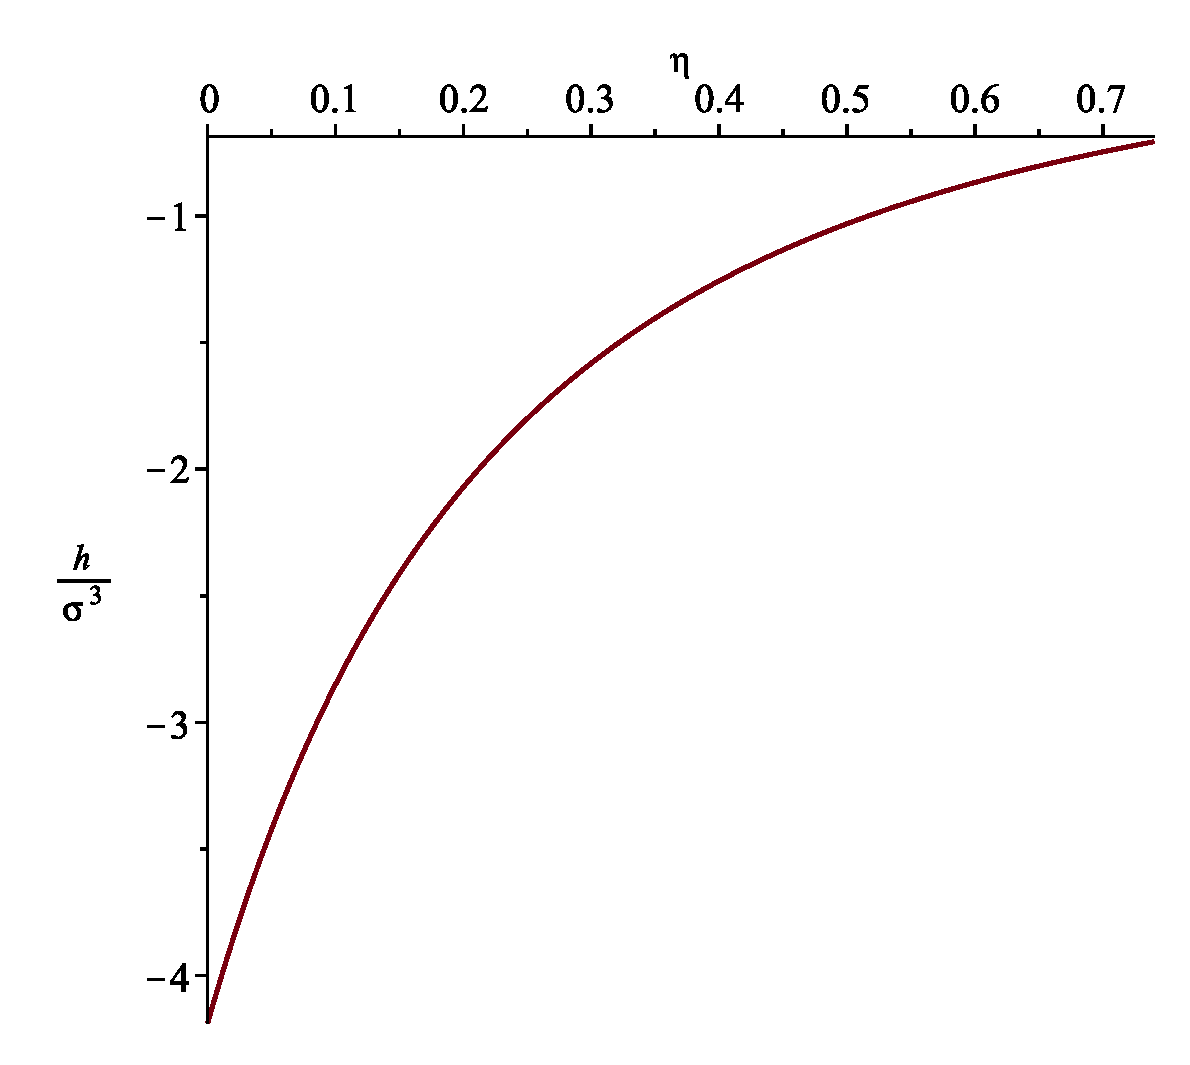
\includegraphics[width=0.45\textwidth,angle=0]{h2_as_function_of_eta_at_k_equals_0} \\
	\parbox{0.5\textwidth}{\caption{\label{h2_vs_k} Fourier transform of the total correlation function $\hat{h}^{(2)}(k)$ divided by the cube of HS diameter $\sigma$ as a function of $k\sigma$ at different values of packing fraction $\eta$. $\eta = 0.05$, $\eta=0.1$, $\eta = 0.15$, and $\eta=0.2$.
	}} \hfill
	\parbox{0.45\textwidth}{\caption{\label{h2_vs_eta} Fourier transform of the total correlation function $\hat{h}^{(2)}(k)$ divided by the cube of HS diameter $\sigma$ as a function of packing fraction $\eta$ at $\vb k = 0$
	}}
\end{figure}

\subsection{Some recurrence relations for correlation functions}
In this section, some recurrence relations for the total correlation functions $h^{(n)}$ will be derived. Let's use equations for the $n$-particle density from~\cite{Schofield1966} (Eq.~(A7) therein):
\begin{equation}
	\frac{\partial\rho^{(n)}}{\partial\rho}\bigg|_T = \frac{n\rho^{(n)} 
		+ \int \{ \rho^{(n+1)}(\vb r_1, \dotsc, \vb r_{n+1}) - \rho^{(n)}(\vb r_1, \dotsc, \vb r_n) \rho^{(1)}(\vb r_{n+1}) \} {\rm d} \vb r_{n+1}}
	{(1/V)\int \rho^{(1)}(\vb r_1) {\rm d} \vb r_1 + \int \{ \rho^{(2)}(\vb r_1, \vb r_2) - \rho^{(1)}(\vb r_1)\rho^{(1)}(\vb r_2) \} {\rm d} \vb r_1}
\end{equation}
which is rewritten in terms of the $n$-particle distribution functions as (Eq.~(A8) in~\cite{Schofield1966})
\begin{equation}
	\label{recur_g}
	\frac{\partial (\rho^n g^{(n)})}{\partial\rho} \bigg|_T 
	= \frac{n\rho^{n-1}g^{(n)} + \rho^n \int \{g^{(n+1)}(\vb r_1, \dots, \vb r_{n+1}) - g^{(n)}(\vb r_1, \dots, \vb r_n)\} {\rm d} \vb r_{n+1}}
	{1 + \rho\int \{g^2(\vb r_1, \vb r_2) - 1\} {\rm d} \vb r_1}
\end{equation}

First, consider $n=2$ and rewrite~(\ref{recur_g}) in terms of correlation functions:
\begin{eqnarray}
	&&\frac{\partial}{\partial\rho}\left(\rho^2 h^{(2)}(\vb r_1, \vb r_2) + \rho^2\right) =
	\nonumber\\
	&&= \frac
	{2\rho(h^{(2)}(\vb r_1, \vb r_2) + 1) + \int \left(h^{(3)}(\vb r_1, \vb r_2, \vb r_3) + h^{(2)}(\vb r_1, \vb r_3) + h^{(2)}(\vb r_2, \vb r_3) \right) {\rm d}{\vb r_3}}
	{1 + \rho \hat{h}^{(2)}(0)}.
\end{eqnarray}
Then apply the following Fourier transformation to the above equation:
\begin{equation}
	\mathcal{F}_2(\dots) = \iint {\rm e}^{-{\rm i}\vb k_1 \vb r_1 - {\rm i} \vb k_2 \vb r_2} \dots {\rm d} \vb r_1 {\rm d} \vb r_2
\end{equation}
As a result, after some algebraic manipulations, the following relations between $\hat{h}^{(3)}$ and $\hat{h}^{(2)}$ are obtained:
\begin{equation}
	\hat{h}^{(3)}(\vb k_1, \vb k_2, 0) = 2 \hat{h}^{(2)}(0)\hat{h}^{(2)}(\vb k_1, \vb k_2) + \frac{\partial \hat{h}^{(2)}(\vb k_1, \vb k_2)}{\partial\rho}(1 + \rho\hat{h}^{(2)}(0)),
\end{equation}
\begin{equation}
	\label{recur_h3_h2}
	\hat{h}^{(3)}(k, -k) = 2 \hat{h}^{(2)}(0)\hat{h}^{(2)}(k) + \frac{\partial \hat{h}^{(2)}(k)}{\partial\rho}(1 + \rho\hat{h}^{(2)}(0)).
\end{equation}

Similarly, the relations between $\hat{h}^{(4)}$ and $\hat{h}^{(3)}$ are as following:
\begin{equation}
	\hat{h}^{(4)}(\vb k_1, \vb k_2, \vb k_3, 0) = 3\hat{h}^{(2)}(0)\hat{h}^{(3)}(\vb k_1, \vb k_2, \vb k_3) + \frac{\partial \hat{h}^{(3)}(\vb k_1, \vb k_2, \vb k_3)} {\partial \rho} (1 + \rho\hat{h}^{(2)}(0)),
\end{equation}
\begin{equation}
	\label{recur_h4_h3}
	\hat{h}^{(4)}(\vb k_1, \vb k_2, 0) = 3\hat{h}^{(2)}(0)\hat{h}^{(3)}(\vb k_1, \vb k_2) + \frac{\partial \hat{h}^{(3)}(\vb k_1, \vb k_2)} {\partial \rho} (1 + \rho\hat{h}^{(2)}(0))
\end{equation}
The relations~(\ref{recur_m3_m2}) and~(\ref{recur_m4_m2}) for cumulants follow directly from~(\ref{recur_h3_h2}) and~(\ref{recur_h4_h3}), respectively.

